% =====================================================================
% 附录 AK《聚变安全与环境：从氚的克数到废物的分级》
% 数值唯一来源：tmp/appAK_calc.py -> tmp/appAK_calc.txt（正文与门禁 P43 只引用该输出）
% 单位写法：数字与单位都进数学模式；单位里带中文时用 \text{}（如 \text{g/年}）
% 分级：现算级（脚本可复算）/ 声明级（脚本顶部输入，正文标明）/ 文献级（只作对照）
% 版权口径：只借鉴结论、公式形式与题型；文字、数值、表格自拟并独立复算；
%           离线环境无法核验 DOI，故只给书名/作者/年份/卷期页
% 与相邻附录的分工：Z 讲工程账、AJ 讲粒子账与氚存量、N 讲材料与壁；
%           本附录只补「安全与环境这本账怎么算」——活度、剂量、活化、废物分级与事故余量
% =====================================================================

\section{第四本账：把安全写成数字}
\label{sec:app-ak-frame}

前面的附录已经算了三本账：能量账（U、Z）、粒子账（AJ）、材料账（N、Z）。
这三本账回答的是「能不能发电、发多少电」。它们都没有回答第四个问题：
\textbf{发出来的这些东西，会不会变成剂量与废物？}

这个问题不能用形容词回答。安全工程的做法是把它拆成两个可以量的自变量：
\textbf{氚的活度}（贝可勒尔）与\textbf{材料的比活度}（贝可每千克）。
只要这两个量算得出来，剂量、释放限值、废物分级、事故余量都是它们的函数。

两个自变量的源头都是中子。D-T 反应放出 14.1 MeV 的中子，
壁上的中子负载 $q_n$ 与中子通量 $\phi$ 的关系只有能量一个因子：

\begin{equation}
\phi=\frac{q_n}{E_n}
=\frac{0.90944\times10^{6}\ \mathrm{W\,m^{-2}}}{14.1\times10^{6}\times1.602176634\times10^{-19}\ \mathrm{J}}
=4.02573\times10^{17}\ \mathrm{n\,m^{-2}\,s^{-1}},
\label{eq:app-ak-flux}
\end{equation}

一年（$3.15576\times10^{7}$ s）的注量是 $1.27042\times10^{25}\ \mathrm{n\,m^{-2}}$。
中子功率占总聚变功率的比例是 $P_n/P_{fus}=445.2/556.5=0.8$，
也就是说 \textbf{80\% 的能量以中子形式穿过第一壁}——这既是发电的本钱，也是活化与氚增殖的来源。

位移损伤用位移截面 $\sigma_d$ 折算。本书不另立一套模型，
而是\textbf{用附录 Z 已经用过的损伤率反推}位移截面，
让两个附录的 dpa 数严格自洽：

\begin{equation}
\sigma_d=\frac{4.5472\ \mathrm{dpa}}{1.27042\times10^{25}\ \mathrm{n\,m^{-2}}}
=3.57928\times10^{-25}\ \mathrm{m^{2}}=3579.28\ \mathrm{b},
\label{eq:app-ak-dpa}
\end{equation}

于是寿期（$10.996$ 年）累计损伤是 $4.5472\times10.996=50.001$ dpa。
注意这里说清了口径：$\sigma_d$ 是\textbf{标定值}，不是独立测量的物理常数。

\begin{table}[htbp]
\centering
\small
\begin{tabular}{p{3.4cm}p{3.3cm}p{3.1cm}p{3.9cm}}
\toprule
量 & 表达式 & 数值 & 说明 \\
\midrule
中子壁负载 & $q_n$ & $0.90944\ \mathrm{MW\,m^{-2}}$ & 附录 Z 口径 \\
中子通量 & $q_n/E_n$ & $4.02573\times10^{17}\ \mathrm{n\,m^{-2}\,s^{-1}}$ & 只差一个中子能量 \\
年注量 & $\phi\times3.15576\times10^{7}$ & $1.27042\times10^{25}\ \mathrm{n\,m^{-2}}$ & 一年累计 \\
位移截面 & 标定 & $3579.28\ \mathrm{b}$ & 与附录 Z 的 $4.5472$ dpa/年 自洽 \\
寿期累计损伤 & $\sigma_d\phi t_{life}$ & $50.001\ \mathrm{dpa}$ & $10.996$ 年 \\
\bottomrule
\end{tabular}
\caption{安全账的两个自变量都从同一个中子通量出发（数值唯一来源 \texttt{tmp/appAK\_calc.py}）。}
\label{tab:app-ak-frame}
\end{table}

\begin{tip}{安全不是感觉，是数字}{tip-app-ak-frame}
「安全」在工程里不是一个形容词，而是一串可以复算的乘式：
活度 $\times$ 剂量系数 $=$ 剂量；释放量 $\times$ 场址因子 $=$ 公众剂量；
比活度 $\div$ 豁免水平 $=$ 废物等级。只要乘式里的每一项都可以被独立复算，
安全论证就不依赖任何人的态度。
\end{tip}

\textbf{出处：}本附录的安全量化框架参照 Dolan（编）\emph{Magnetic Fusion Technology}（2013，安全与氚处理章节）、
Tanabe（编）\emph{Tritium: Fuel of Fusion Reactors}（2017，第 1、4 章）、
IAEA \emph{Safety of Fusion Facilities} 系列技术文件（1990 年代起）；
中子学与损伤量的口径与附录 Z、N 保持一致。本节凡标出数字的量都由 \texttt{tmp/appAK\_calc.py} 复算。

\section{氚的活度与剂量：克数怎么变成西弗}
\label{sec:app-ak-tritium}

公众听到「堆里有 2 千克氚」时无法判断严重程度，因为质量不是剂量的单位。
中间要过两道换算：\textbf{质量 $\to$ 活度}（贝可）与\textbf{活度 $\to$ 剂量}（西弗）。

第一道换算只依赖半衰期。氚的半衰期是 12.32 年，衰变常数
$\lambda=\ln 2/T_{1/2}=1.78283\times10^{-9}\ \mathrm{s^{-1}}$，
1 g 氚含 $1.9967\times10^{23}$ 个原子，于是比活度是：

\begin{equation}
\begin{aligned}
a_T&=\lambda\,\frac{m}{m_T}\\
&=1.78283\times10^{-9}\times\frac{10^{-3}}{3.0160492\times1.66053906660\times10^{-27}}\\
&=3.55978\times10^{14}\ \mathrm{Bq\,g^{-1}}=355.978\ \mathrm{TBq\,g^{-1}}.
\end{aligned}
\label{eq:app-ak-activity}
\end{equation}

由这个数出发，任何质量都能立刻换算：1 mg 是 $3.55978\times10^{11}$ Bq，
0.1 g 是 $3.55978\times10^{13}$ Bq，附录 AJ 与 Z 用的库存上限 2 kg 是

\begin{equation}
A_{inv}=3.55978\times10^{14}\times2000=7.11956\times10^{17}\ \mathrm{Bq}.
\label{eq:app-ak-inventory}
\end{equation}

第二道换算依赖\textbf{摄入途径}，而不是距离。氚的 $\beta$ 粒子平均能量只有 5.7 keV，
在空气中走不到 6 mm，在皮肤里走不到 1 $\mu$m——\textbf{外照射几乎可以忽略}。
危险全在摄入：氚水（HTO）在体内与水同路，生物半衰期约 10 天，
于是吸入 1 Bq 的待积有效剂量系数是 $1.8\times10^{-11}$ Sv/Bq（ICRP 量级，声明值）：

\begin{equation}
D=A\times d_{HTO}=3.55978\times10^{14}\times1.8\times10^{-11}
=6407.61\ \mathrm{Sv}.
\label{eq:app-ak-dose}
\end{equation}

也就是说，\textbf{1 克氚全部氧化后被一个人吸入，相当于 6400 西弗}——
限值的六千倍。反过来问才有工程意义：拿到 1 mSv 需要多少？

\begin{equation}
A_{1\,\mathrm{mSv}}=\frac{10^{-3}}{1.8\times10^{-11}}
=5.55556\times10^{7}\ \mathrm{Bq}=1.56065\times10^{-7}\ \mathrm{g}=0.156065\ \mu\mathrm{g}.
\label{eq:app-ak-limit}
\end{equation}

\textbf{亚微克量级}。这就是为什么氚安全的所有工程手段都朝向同一个方向：
不要让它以氚水的形式进入人体。作为对照，职业限值 20 mSv 对应
$1.11111\times10^{9}$ Bq，即 $3.12129\times10^{-6}$ g——仍然只有 3 微克。

化学形态的影响同样巨大：若氚以 HT 气体形式存在，
剂量系数是 $1.8\times10^{-15}$ Sv/Bq，同样 1 g 的剂量只有 $0.640761$ Sv，
\textbf{比 HTO 低 10000 倍}。最后把这条链推到年尺度：燃耗 $31.191$ kg/年
是 $1.11033\times10^{19}$ Bq/年，

\begin{equation}
D_{1\%}=1.11033\times10^{19}\times0.01\times1.8\times10^{-11}
=1.9986\times10^{6}\ \mathrm{Sv},
\label{eq:app-ak-burn}
\end{equation}

即\textbf{年燃耗的 1\% 若全部以氚水形式被一个人吸入，剂量是百万西弗量级}。
这个数不是用来吓人的，而是用来说明包容与除氚为什么是设计要求而不是可选项。

\begin{table}[htbp]
\centering
\small
\begin{tabular}{p{2.7cm}p{3.6cm}p{3.1cm}p{4.3cm}}
\toprule
质量 & 活度 & 全吸入剂量 & 说明 \\
\midrule
1 mg & $3.55978\times10^{11}\ \mathrm{Bq}$ & $6.40761\ \mathrm{Sv}$ & 一滴水的千分之一 \\
0.1 g & $3.55978\times10^{13}\ \mathrm{Bq}$ & $640.761\ \mathrm{Sv}$ & 仍远超限值 \\
1 g & $3.55978\times10^{14}\ \mathrm{Bq}$ & $6407.61\ \mathrm{Sv}$ & 公众限值的六千倍 \\
2 kg（库存上限） & $7.11956\times10^{17}\ \mathrm{Bq}$ & $1.28152\times10^{7}\ \mathrm{Sv}$ & 附录 Z/AJ 口径 \\
31.191 kg（年燃耗） & $1.11033\times10^{19}\ \mathrm{Bq}$ & $1.9986\times10^{8}\ \mathrm{Sv}$ & 只算 1\% 也有百万西弗 \\
\bottomrule
\end{tabular}
\caption{氚的质量、活度与剂量阶梯（剂量系数取 HTO 吸入 $1.8\times10^{-11}$ Sv/Bq，声明值；全吸入是上界口径）。}
\label{tab:app-ak-tritium}
\end{table}

\begin{tip}{氚的危险不在外照射，在摄入}{tip-app-ak-tritium}
氚的 $\beta$ 在皮肤里走不到 1 $\mu$m，站在 2 kg 氚旁边不会受到外照射伤害；
但 0.156 $\mu$g 的氚水就够 1 mSv。安全设计因此不围着「屏蔽」转，
而围着\textbf{密封、通风、除氚与个人监测}转——能量的形态决定了防护的形态。
\end{tip}

\textbf{出处：}氚的比活度与剂量换算参照 Tanabe（编）\emph{Tritium: Fuel of Fusion Reactors}（2017，第 2--3 章）、
ICRP 第 72 号出版物（1996，氚的剂量系数）与第 103 号出版物（2007，剂量限值体系）、
Turner \emph{Atoms, Radiation, and Radiation Protection}（2007，第 8--9 章）。本节凡标出数字的量都由 \texttt{tmp/appAK\_calc.py} 复算。

\section{氚的包容：渗透、除氚与年释放目标}
\label{sec:app-ak-containment}

氚不会老老实实待在管道里。它是最轻的元素，会溶解进金属、沿晶格扩散、
从外表面重新组合成分子跑掉——这个过程叫\textbf{渗透}。
渗透通量正比于壁两侧氚分压的平方根、反比于壁厚，工程上用\textbf{渗透降低因子}
（PRF）描述屏障的贡献：

\begin{equation}
j=\frac{j_0}{\mathrm{PRF}}
=\frac{10^{9}}{100}=10^{7}\ \mathrm{Bq\,m^{-2}\,s^{-1}}.
\label{eq:app-ak-perm}
\end{equation}

其中 $j_0=10^{9}$ Bq\,m$^{-2}$\,s$^{-1}$ 是无屏障时的通量（文献量级，声明值），
PRF $=100$ 是带屏障的典型值（声明值）。乘上附录 X 用过的第一壁面积
$489.532$ m$^{2}$，全天候渗透率是 $4.89532\times10^{9}$ Bq/s，
折合 $1.18815$ g/天、$0.433972$ kg/年——
\textbf{相当于燃耗的 $1.39134\%$}。

接下来是关键的一步：把它与允许的释放量比。工程上通常把氚的年释放目标
定在 1 g/年（文献量级，声明值），即 $3.55978\times10^{14}$ Bq/年。
于是所需的除氚因子是

\begin{equation}
\mathrm{DF_{need}}=\frac{4.22956\times10^{14}}{3.55978\times10^{14}}=433.972,
\label{eq:app-ak-df}
\end{equation}

也就是说\textbf{屏障与除氚系统必须再把这股氚流压小四百多倍}，
才能让它落在管理目标之内。另一条独立的线来自附录 AJ：
加料氚流 $162.72$ kg/年 的 1\% 滞留是 $1.6272$ kg/年，
而库存上限 2 kg 意味着这份滞留最多只能攒 $1.22911$ 年——
\textbf{渗透管的是「跑出去多少」，滞留管的是「攒下来多少」，两笔账都不能省}。

除氚系统的时间常数可以用一级去除估计。手套箱 $1000$ m$^{3}$，
初始浓度 $10^{6}$ Bq/m$^{3}$，目标 $10^{3}$ Bq/m$^{3}$，
去除速率常数 $1$ h$^{-1}$（声明值）：

\begin{equation}
t=\frac{\ln(A_0/A_1)}{k}=\frac{\ln 1000}{1}=6.90776\ \mathrm{h}.
\label{eq:app-ak-clean}
\end{equation}

浓度比 1000 需要 $6.90776$ 个时间常数——这就是「除氚因子」这个词的来源：
它本质上是\textbf{浓度比的对数}，不是效率的百分比。

\begin{table}[htbp]
\centering
\small
\begin{tabular}{p{2.9cm}p{3.5cm}p{3.2cm}p{4.1cm}}
\toprule
出路 & 数值 & 与管理目标之比 & 对策 \\
\midrule
壁渗透 & $0.433972$ kg/年 & $433.972$ 倍 & 渗透屏障 + 除氚 \\
滞留（AJ 口径） & $1.6272$ kg/年 & 库存 2 kg 只够 $1.22911$ 年 & 氚工厂回收 \\
事故释放 & 释放份额 $0.1$ & 见 \S AK.6 & 安全壳 + 纵深防御 \\
\bottomrule
\end{tabular}
\caption{氚的三条出路各有各的量纲，但都能折成「与 1 g/年 目标之比」这一把尺子。}
\label{tab:app-ak-containment}
\end{table}

\begin{tip}{屏障不是可选项，是设计输入}{tip-app-ak-containment}
渗透不是「漏」，而是材料在热力学上必然发生的过程：只要壁两侧有氚分压差，
氚就会穿过去。因此屏障、载气除氚、手套箱与通风都不是附加设备，
而是\textbf{决定了堆能不能拿到许可}的设计输入——把 PRF 从 100 提到 1000，
渗透量就按比例下降，这一条在练习 3 里复算。
\end{tip}

\textbf{出处：}氚渗透与除氚的工程口径参照 Tanabe（编）\emph{Tritium: Fuel of Fusion Reactors}（2017，第 4--6 章）、
Dolan（编）\emph{Magnetic Fusion Technology}（2013，氚系统章节）、
ITER 氚处理系统的公开设计描述（2000 年代）。本节凡标出数字的量都由 \texttt{tmp/appAK\_calc.py} 复算。
\section{中子活化：壁材料怎么变成放射性废物}
\label{sec:app-ak-activation}

氚是燃料带来的问题，活化是\textbf{中子带来的第二份产物}。
14.1 MeV 的中子打进钢里，会把稳定的原子核打成放射性核素；
材料的化学成分没有变，但它的「身份」变了——从结构材料变成了放射性废物。

活化的第一步是把通量积成注量。第一壁每年接受的中子注量是

\begin{equation}
\Phi=\phi\,t=4.02573\times10^{17}\times3.15576\times10^{7}
=1.27042\times10^{25}\ \mathrm{n\,m^{-2}},
\label{eq:app-ak-fluence}
\end{equation}

用 \S AK.1 标定的位移截面折算，就是附录 Z 已经用过的 $4.5472$ dpa/年，
寿期累计 $50.001$ dpa。位移损伤之外还有气体产物：若氦产额按
$10$ appm/dpa 计（声明值），寿期累计约 $500.01$ appm 的氦——
这就是材料会变脆、会起泡的原因，附录 N 已从材料角度讨论过。

废物账要看的是活度，而不是 dpa。工程上常用的办法是直接给出
\textbf{寿期末的比活度}：对典型堆内构件取 $10^{6}$ Bq/kg（文献量级，声明值）。
待处置构件 $10^{6}$ kg（声明值），金属密度 $7800$ kg/m$^{3}$：

\begin{equation}
A_{waste}=a_{spec}\,M=10^{6}\times10^{6}=10^{12}\ \mathrm{Bq}=1\ \mathrm{TBq},
\label{eq:app-ak-specact}
\end{equation}

对应体积 $128.205$ m$^{3}$。这个活度是钢的豁免水平
$10^{4}$ Bq/kg（文献量级，声明值）的 $100$ 倍——
\textbf{它不能当普通废钢处理，但也不是高放废物}。分级的门槛在哪里，下一节算。

\begin{table}[htbp]
\centering
\small
\begin{tabular}{p{3.2cm}p{3.4cm}p{3.2cm}p{3.9cm}}
\toprule
量 & 表达式 & 数值 & 说明 \\
\midrule
年注量 & $\phi t$ & $1.27042\times10^{25}$ n\,m$^{-2}$ & 与 $q_n$ 同源 \\
位移损伤 & 标定 $\sigma_d$ & $50.001$ dpa & $10.996$ 年 \\
氦产额 & $10$ appm/dpa & $500.01$ appm & 声明值 \\
比活度（寿期末） & 声明 & $10^{6}$ Bq/kg & 典型堆内构件 \\
总活度 & $a_{spec}M$ & $10^{12}$ Bq & $10^{6}$ kg 构件 \\
豁免水平之比 & $a_{spec}/a_{clear}$ & $100$ 倍 & 需分级处置 \\
\bottomrule
\end{tabular}
\caption{活化链的六个量：注量 $\to$ dpa $\to$ 氦 $\to$ 比活度 $\to$ 总活度 $\to$ 与豁免水平之比。}
\label{tab:app-ak-activation}
\end{table}

\begin{tip}{活化是中子的第二份产物}{tip-app-ak-activation}
中子既是能量的载体，也是「污染源」：同一批中子在包层里造氚、在钢里造放射性核素。
因此聚变堆的废物问题不是运行事故的后果，而是\textbf{正常运行就会产生}的——
它必须在中子学设计阶段就被算出来，而不是在退役时才发现。
\end{tip}

\textbf{出处：}中子活化与废物评价的框架参照 Dolan（编）\emph{Magnetic Fusion Technology}（2013，活化与废物章节）、
Wu \emph{Fusion Neutronics}（2017，第 6--8 章）、
Gilbert 与 Sublet 关于聚变材料活化计算的公开综述（2010 年代）；
位移损伤与 dpa 口径沿用附录 Z 与 N。本节凡标出数字的量都由 \texttt{tmp/appAK\_calc.py} 复算。

\begin{figure}[htbp]
\centering
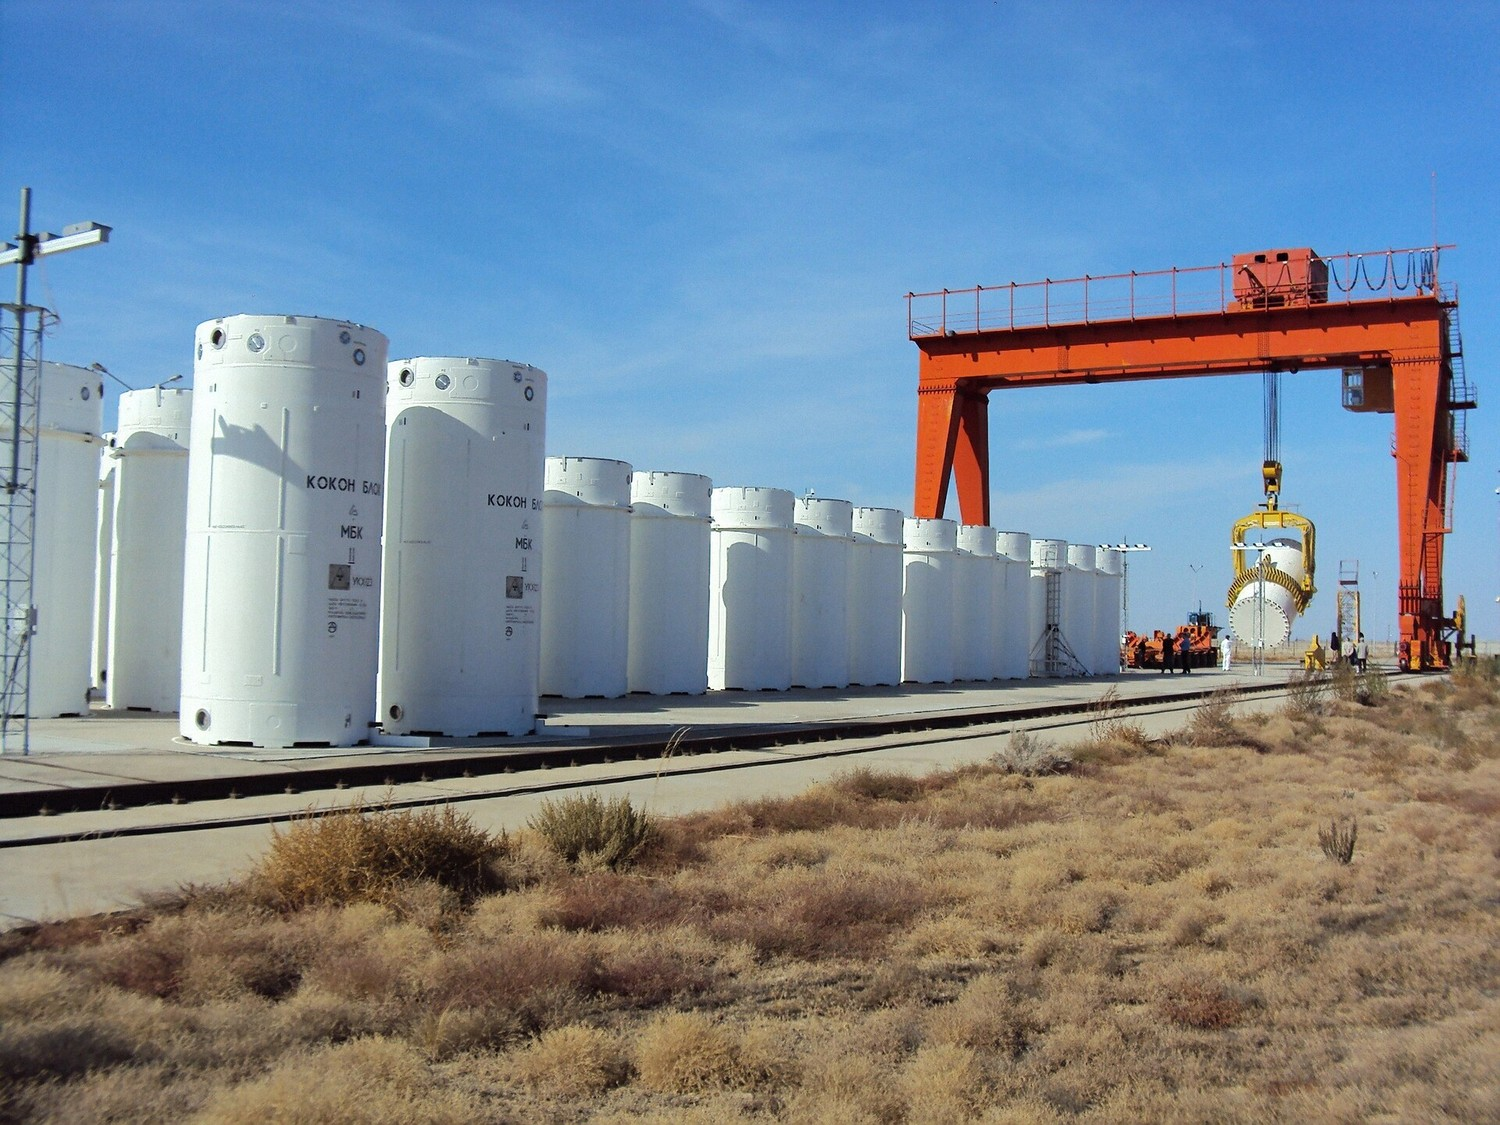
\includegraphics[width=0.78\textwidth]{../figures/dry_cask.jpg}
\caption{活化废物的去处：干式贮存罐。中子活化过的部件最终要装进这样的罐子里：先等衰变热降下来，再按活度分级决定处置方式——本节算的冷却时间与豁免限值，决定了它什么时候能离开厂房。}
\label{fig:photo-appak2}
\figsource{Nuclear Regulatory Commission from US，CC BY 2.0（Wikimedia Commons），链接见 figures/CREDITS.md。}
\end{figure}

\section{衰变热与废物分级：冷却多久才能豁免}
\label{sec:app-ak-waste}

放射性核素的活度按指数衰减。主导堆内构件剂量的是 Co-60 这类中长寿命核素，
半衰期 $5.2711$ 年，衰变常数 $\lambda_{Co}=4.16697\times10^{-9}$ s$^{-1}$：

\begin{equation}
A(t)=A_0e^{-\lambda_{Co}t}.
\label{eq:app-ak-decay}
\end{equation}

废物分级用的第一把尺子是比活度。要让 $10^{6}$ Bq/kg 降到豁免水平
$10^{4}$ Bq/kg，需要

\begin{equation}
t_{clear}=\frac{\ln(A_0/A_{clear})}{\lambda_{Co}}
=\frac{\ln 100}{4.16697\times10^{-9}}=35.0204\ \text{年}.
\label{eq:app-ak-clear}
\end{equation}

冷却 $50$ 年后比活度是 $1394.84$ Bq/kg，即豁免水平的 $0.139484$ 倍——
\textbf{可以申请解控}；冷却 $100$ 年后只剩 $1.94557$ Bq/kg。
注意这中间有一个陡峭的门槛：$35$ 年时刚好压在线上，$50$ 年已经低了一个量级。
分级因此不是「材料好不好」的问题，而是\textbf{冷却时间够不够}的问题。

第二把尺子是衰变热。停机瞬间，$10^{6}$ kg 构件按 $0.05$ W/kg（声明值）
放出 $50$ kW；这些热必须靠自然对流或强制冷却带走，否则包壳会升温。

\begin{equation}
P_{decay}(t)=P_0e^{-\lambda_{Co}t},\qquad
P_0=0.05\times10^{6}=5\times10^{4}\ \mathrm{W}=50\ \mathrm{kW},
\label{eq:app-ak-heat}
\end{equation}

$50$ 年后衰变热降到 $69.7419$ W，衰减 $716.929$ 倍。
分级与储存方案要同时满足两个约束：\textbf{比活度低于豁免水平、衰变热低于散热能力}。

\begin{table}[htbp]
\centering
\small
\begin{tabular}{p{2.6cm}p{3.4cm}p{3.0cm}p{4.4cm}}
\toprule
冷却时间 & 比活度 & 衰变热 & 结论 \\
\midrule
$0$ 年 & $10^{6}$ Bq/kg & $50$ kW & 必须主动冷却 \\
$35.0204$ 年 & $10^{4}$ Bq/kg & —— & 刚压到豁免线 \\
$50$ 年 & $1394.84$ Bq/kg & $69.7419$ W & 可申请解控 \\
$100$ 年 & $1.94557$ Bq/kg & —— & 远低于豁免线 \\
\bottomrule
\end{tabular}
\caption{比活度与衰变热同时衰减，两者共同决定废物的等级与储存时间（Co-60 主导，声明口径）。}
\label{tab:app-ak-waste}
\end{table}

\begin{tip}{废物的等级不是材料定的，是活度定的}{tip-app-ak-waste}
同一吨钢，运行前是普通钢材，寿期后是中放废物，冷却 50 年后可能变成可解控废物。
分级取决于\textbf{此刻的比活度}，因此「退役废物」不是一个固定标签，
而是一条随时间下降的曲线；工程上能做的，是把这条曲线算准、把储存方案排好。
\end{tip}

\textbf{出处：}衰变热与废物分级方法参照 Dolan（编）\emph{Magnetic Fusion Technology}（2013，废物管理章节）、
IAEA 放射性废物分类与解控水平的一般原则（1990 年代起的技术文件）、
Turner \emph{Atoms, Radiation, and Radiation Protection}（2007，第 4--5 章）。本节凡标出数字的量都由 \texttt{tmp/appAK\_calc.py} 复算。

\section{事故与纵深防御：LOCA 情景的剂量账}
\label{sec:app-ak-accident}

安全论证最怕的不是「会不会出事」，而是「出事之后到人多少剂量」。
把这个问题写成乘式，需要三个因子：\textbf{库存、释放份额、环境输运}。

环境输运在工程上打包成一个系数：场址剂量因子 $f$，
即每释放 1 Bq 氚对应的公众剂量。本书用一条公开的量级关系标定它：
1 g 氚释放到大气对应约 $20$ $\mu$Sv（文献量级，声明值），于是

\begin{equation}
f=\frac{20\times10^{-6}}{3.55978\times10^{14}}=5.61832\times10^{-20}\ \mathrm{Sv\,Bq^{-1}}.
\label{eq:app-ak-site}
\end{equation}

事故情景取冷却剂丧失（LOCA）：堆内氚库存 $7.11956\times10^{17}$ Bq（2 kg），
其中 $10\%$ 进入安全壳（声明值），

\begin{equation}
A_{rel}=0.1\times7.11956\times10^{17}=7.11956\times10^{16}\ \mathrm{Bq}=200\ \mathrm{g}.
\label{eq:app-ak-release}
\end{equation}

\textbf{若没有包容}，这 200 g 直接排到边界，公众剂量是
$7.11956\times10^{16}\times5.61832\times10^{-20}=0.004$ Sv $=4$ mSv——
\textbf{是 1 mSv 限值的 4 倍}。这个数说明：一次「无包容」的氚释放事故，
后果不是灾难性的，但足以超标。

\textbf{若包容有效}，安全壳事件期泄漏份额 $10^{-3}$、排放前除氚后剩余 $10^{-2}$
（两项都是声明值），环境释放降到 $7.11956\times10^{11}$ Bq（$0.002$ g），剂量

\begin{equation}
D_{contain}=7.11956\times10^{11}\times5.61832\times10^{-20}
=4\times10^{-8}\ \mathrm{Sv}=0.04\ \mu\mathrm{Sv},
\label{eq:app-ak-margin}
\end{equation}

即限值的 $4\times10^{-5}$，\textbf{余量 25000 倍}。同样的库存、同样的释放份额，
包容让剂量降低了 $100000$ 倍——这就是纵深防御的全部含义：
它不是一道屏障，而是\textbf{一串相乘的因子}。

\begin{table}[htbp]
\centering
\small
\begin{tabular}{p{2.8cm}p{3.3cm}p{3.1cm}p{4.2cm}}
\toprule
环节 & 表达式 & 数值 & 说明 \\
\midrule
堆内库存 & 2 kg & $7.11956\times10^{17}$ Bq & 附录 Z/AJ 口径 \\
进入安全壳 & $10\%$ & $7.11956\times10^{16}$ Bq & 释放份额声明值 \\
无包容剂量 & $A_{rel}f$ & $4$ mSv & 超限值 4 倍 \\
有包容剂量 & $A_{rel}f\times10^{-5}$ & $0.04$ $\mu$Sv & 限值的 $4\times10^{-5}$ \\
余量 & $1\ \mathrm{mSv}/D$ & $25000$ 倍 & 纵深防御的效果 \\
\bottomrule
\end{tabular}
\caption{事故剂量账的三个乘数：库存、释放份额、包容因子；每减少一个量级，余量就多十倍。}
\label{tab:app-ak-accident}
\end{table}

\begin{tip}{纵深防御是乘法，不是加法}{tip-app-ak-accident}
「多一道屏障」在安全论证里不是加一项，而是乘一个因子：
$10^{-1}$（释放份额）$\times10^{-3}$（泄漏）$\times10^{-2}$（除氚）$=10^{-6}$。
所以工程上真正有效的做法，是找出乘式里最大的那一项去压——
在本例中，最先要压的是「进入安全壳的份额」，而不是再加一层钢板。
\end{tip}

\textbf{出处：}事故情景与包容设计参照 Dolan（编）\emph{Magnetic Fusion Technology}（2013，安全分析章节）、
ITER 安全分析报告公开摘要（2000 年代）、
IAEA 聚变设施安全标准系列（1990 年代起）；场址剂量因子按公开量级关系标定（声明值）。本节凡标出数字的量都由 \texttt{tmp/appAK\_calc.py} 复算。

\section{估算练习}
\label{sec:app-ak-problems}

六道题都用工况点（附录 Z/AJ 同一台堆）与前面各节的公式；
需要改动参数时以题面给出的数值为准，并说明与工况点相比变化了几倍。

\textbf{练习 1}实验室里有一小瓶 10 mg 的氚水。它的活度是多少贝可？
若全部被一个人吸入，剂量是多少西弗？与公众限值比呢？

\textbf{练习 2}同样用 HT 气体的剂量系数（$1.8\times10^{-15}$ Sv/Bq）计算：
1 mSv 对应摄入多少贝可、多少克？与 HTO 相比宽了多少倍？

\textbf{练习 3}若把渗透屏障的 PRF 从 100 提到 1000，全壁渗透率变成多少，
折合每天、每年多少克？还需要多大的除氚因子？

\textbf{练习 4}若堆内氚库存是 1 kg，事故释放份额仍是 10\%，
包容因子与本节相同（$10^{-5}$），环境释放量与公众剂量各是多少？

\textbf{练习 5}若把解控的目标放宽到豁免水平的 10 倍（$10^{5}$ Bq/kg），
冷却时间可以缩短到多少年？

\textbf{练习 6}若氦产额取 5 appm/dpa（而不是 10 appm/dpa），
寿期累计氦浓度是多少？这说明材料评价对哪一个输入最敏感？

\textbf{解答 1}活度 $=3.55978\times10^{12}$ Bq $=3559.78$ GBq$=3.55978$ TBq；
剂量 $=3.55978\times10^{12}\times1.8\times10^{-11}=64.0761$ Sv，
是公众限值的 $64076.1$ 倍。

\textbf{解答 2}摄入 $=10^{-3}/1.8\times10^{-15}=5.55556\times10^{11}$ Bq
$=0.00156065$ g $=1.56065$ mg；比 HTO 宽 $10000$ 倍（正好是两种剂量系数之比）。

\textbf{解答 3}$j=10^{9}/1000=10^{6}$ Bq\,m$^{-2}$\,s$^{-1}$；
全壁 $10^{6}\times489.532=4.89532\times10^{8}$ Bq/s，
折合 $0.118815$ g/天、$0.0433972$ kg/年，
与管理目标 1 g/年 之比 $43.3972$ 倍——除氚因子只需 $43.3972$。

\textbf{解答 4}库存 1 kg 的活度 $3.55978\times10^{14}\times1000=3.55978\times10^{17}$ Bq；
释放 10\% 后乘 $10^{-5}$，环境释放 $3.55978\times10^{11}$ Bq；
剂量 $=3.55978\times10^{11}\times5.61832\times10^{-20}=2\times10^{-8}$ Sv $=0.02$ $\mu$Sv。

\textbf{解答 5}$t=\ln(10^{6}/10^{5})/4.16697\times10^{-9}=17.5102$ 年，
比 $35.0204$ 年短一半——因为指数衰减的「半衰期式」压缩：
目标放宽 10 倍只省下 17.5 年，但门槛附近的这 17.5 年决定了储存设施要不要建。

\textbf{解答 6}寿期累计氦 $=5\times50.001=250.005$ appm，正好是 $10$ appm/dpa 情形的一半。
材料评价因此对\textbf{氦产额与位移截面两个输入同样敏感}：
两者都来自中子能谱与核数据，说明「核数据」是安全与材料论证的共同底座。

\section{来源、分级与版权说明}
\label{sec:app-ak-source}

本附录的数值分三级，阅读时请按级取用。

\begin{table}[htbp]
\centering
\small
\begin{tabular}{p{2.3cm}p{3.5cm}p{5.2cm}p{2.6cm}}
\toprule
级别 & 含义 & 本附录中的例子 & 可否复算 \\
\midrule
现算级 & 由脚本按公式算出 & $3.55978\times10^{14}$ Bq/g、$6407.61$ Sv、$35.0204$ 年、$25000$ 倍 & 可以 \\
声明级 & 脚本顶部的输入 & 剂量系数 $1.8\times10^{-11}$ Sv/Bq、比活度 $10^{6}$ Bq/kg、PRF $=100$ & 改输入即可 \\
文献级 & 只作量级对照 & 年释放目标 1 g/年、场址因子 $20$ $\mu$Sv/g、豁免水平 $10^{4}$ Bq/kg & 不做断言 \\
\bottomrule
\end{tabular}
\caption{三级数值口径。凡正文未标注「声明」或「文献量级」的数字，都属于现算级。}
\label{tab:app-ak-source}
\end{table}

\textbf{不复制}：本附录不复制任何原教材的文字、编号、插图与数据表；
只借鉴其结论、公式形式与题型，全部文字、数值与表格自拟并独立复算。

\textbf{不复制}：不复制任何核数据库、活化计算程序（如 FISPACT 类）的输出表格；
本附录只用可复算的标定量级。

\textbf{不复制}：不复制任何监管文件的具体限值与许可证条款文本；
剂量限值只按 ICRP 公开体系引用数量级。

\textbf{不复制}：不复制任何场址的大气弥散计算书；
场址剂量因子只用公开量级关系标定，并在正文标明为声明值。

\textbf{不复制}：不复制任何厂商的氚系统设计与材料渗透数据表；
渗透与除氚均按声明量级给出，练习中改动 PRF 只为演示标度关系。

\begin{tip}{本附录不给什么}{tip-app-ak-honest}
本附录不给三样东西：\textbf{不给场址级的大气弥散与剂量评价}（那需要气象、地形与源项数据），
\textbf{不给核数据的原始评价}（那需要评价数据库与活化程序），
\textbf{不给监管判断}（那是许可证审评机构的事）。
它只做一件事：把安全论证里最容易含糊的那几个乘式，
用同一台堆的数字算成可以复算的量。
\end{tip}

\textbf{出处：}本附录的三级口径与版权处理沿用附录 K、L、N、Z 的约定；
剂量体系参照 ICRP 第 72 号（1996）与第 103 号（2007）出版物，
氚与活化工程口径参照 Dolan（编）\emph{Magnetic Fusion Technology}（2013）与
Tanabe（编）\emph{Tritium: Fuel of Fusion Reactors}（2017），
废物分级参照 IAEA 公开技术文件。离线环境无法核验 DOI，故只给书名、作者、年份与章节。
